%!TEX root = ../thesis.tex
\chapter{Data}
\label{chap:data}


\section{Data Information}

\subsection{Data Tables}
\begin{enumerate}
    \item "TickerName": stock market data from eodhistoricaldata and are in json format, shown in figure 3.2 includes symbol, date, open, high, low, close, adjusted close, volume from 2014-01-01 to recent, where only adjusted close price is used in our trading model.
    \item "sp500": SP500 constituent data from pkgstore.datahub.io in json format, shown in figure 3.1, which includes name, sector and symbol.
    \item "stockpairs": stock pairs constituent data from training model, which includes ticker1 and ticker2 in pairs, score that represent the strength of cointegration, profit and loss for the pair in backtesting.
    \item "pairprices": stock pairs price data with adjusted close price of each pair from stock market data, residuals from pair prices regression, and bollinger band constructed from residuals.
    \item "trades": trades data that record pair, date, price, quantity and PnL of trade status everyday.
\end{enumerate}

\subsection{Data Retrieval}
We first put SP500 constituent data into database, then retrieve data from each ticker from SP500 and also SP500 index price.

\begin{figure}
\centering
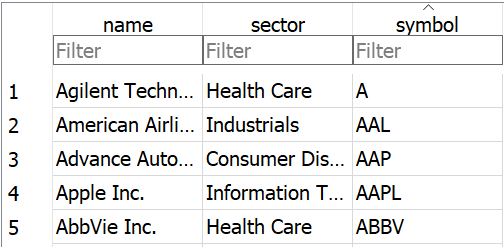
\includegraphics[scale=0.6]{data/images/sp500table.png}
\caption{Table: SP500 Constituents}
\label{fig:sp500}
\end{figure}

\begin{figure}
\centering
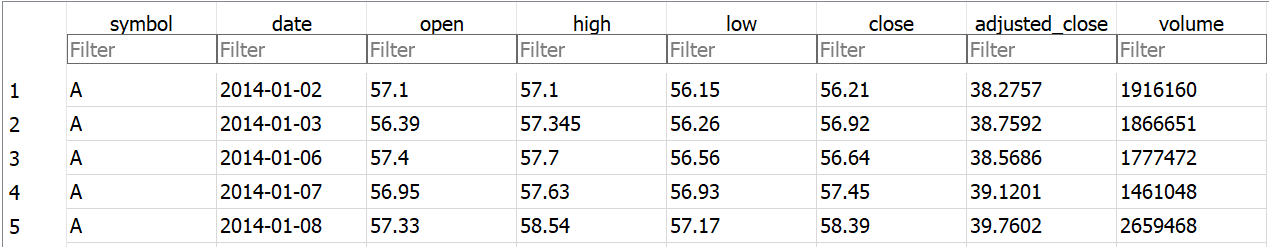
\includegraphics[scale=0.6]{data/images/A.png}
\caption{Table: Stock A}
\label{fig:stockA}
\end{figure}

Function get\_daily\_data() takes in ticker name, start date, end date, data url, api key to get market data for one stock starting from start date to end date. Python packpage urlopen is used to open url and data is parsed from json format to dictionary then to pandas dataframe in Function download\_stock\_data(). Then, the dataframe is stored in SQLite in this function. These functions are shown in Figure 3.3 and 3.4.

\begin{figure}
\centering
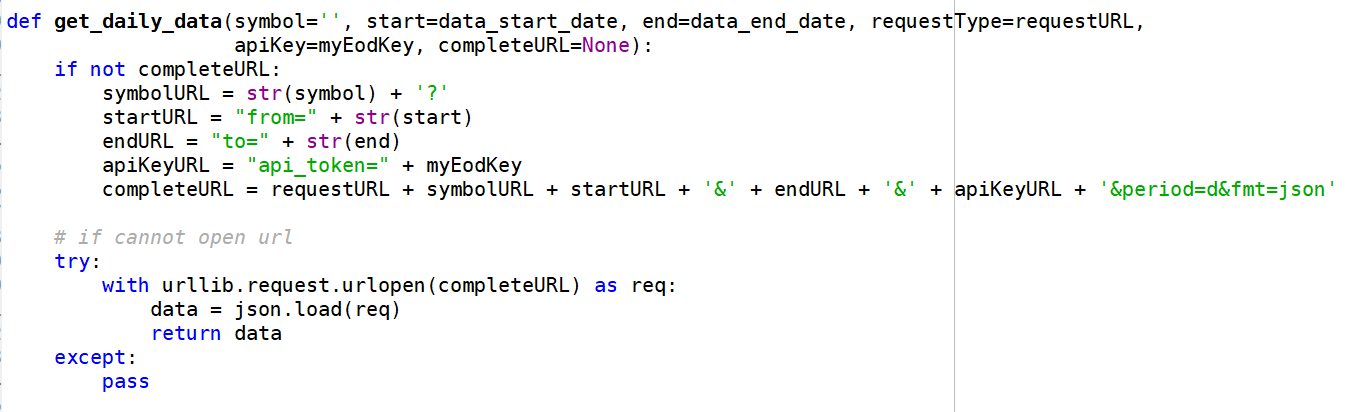
\includegraphics[scale=0.6]{data/images/getdailydata.png}
\caption{Function: get\_daily\_data()}
\label{fig:getdailydata}
\end{figure}

\begin{figure}
\centering
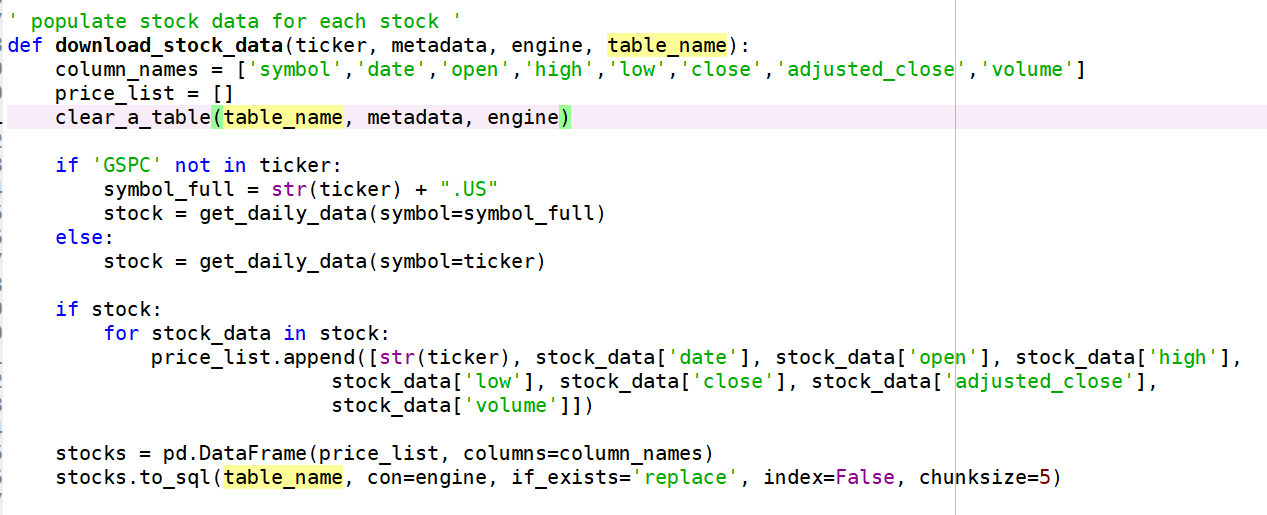
\includegraphics[scale=0.6]{data/images/downloaddata.png}
\caption{Function: download\_stock\_data()}
\label{fig:downloaddata}
\end{figure}


\section{Database Design}

Our database design comprises of 504 tables with two entity relationship, as shown in Figure 3.1. First, each of 500 ticker database with "symbol" and "date" as primary key and "symbol" as foreign key maps to "name" as primary key from sp500 constituents database. Second, table "pairprices" and table "trades" both have "symbol1", "symbol2" that reference to "ticker1", "ticker2" in table stockpairs.

\begin{figure}[h!]
\centering
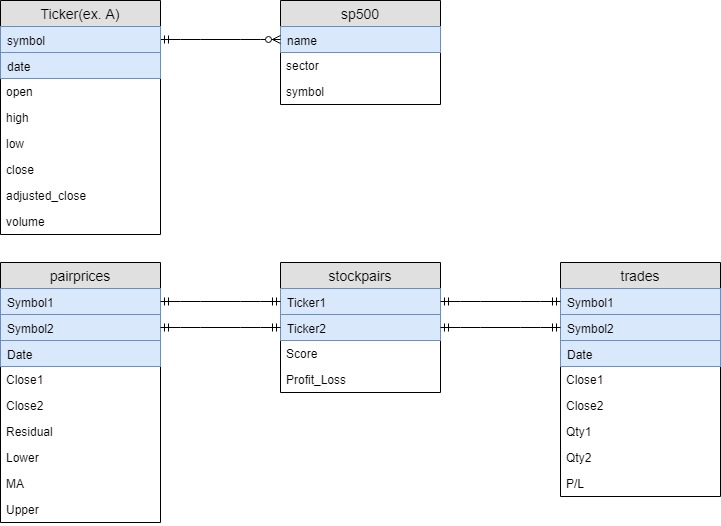
\includegraphics[scale=0.45]{data/images/database.jpg}
\caption{Database Design}
\label{fig:database}
\end{figure}